\chapter{Interest Rate Derivatives}
\label{interest-rate-swaps-and-swaptions}

In Chapter~\ref{sec:swaps-and-bootstrapping} we introduced the Overnight Index Swap, a particular type of swap. Here we describe the plain vanilla Interest Rate Swap contract and see how it can underlie a Swaption, the European options analogous for interest rate market.

\section{Interest Rate Swaps}\label{interest-rate-swaps}

Interest rate swaps (IRS) consist of two legs. The floating leg pays the reference index fixing at a frequency equal to the floating rate tenor, so for example an IRS on a 3-month EURIBOR will pay a floating coupon every three months.
The fixed leg pays a predetermined cash-flow at annual frequency, regardless of the underlying floating rate tenor (for simplicity we will only consider swaps with maturities which are multiples of 1 year).

The contract parameters are:

\begin{itemize}
\tightlist
\item start date $d_0$;
\item notional $N$;
\item fixed rate $K$;
\item floating rate tenor (months);
\item maturity (years).
\end{itemize}

\subsection{IRS Valuation}
\label{irs-valuation}

Let $d_0^{\mathrm{fixed}},...,d_p^{\mathrm{fixed}}$ be the fixed leg payment dates and $d_0^{\mathrm{float}},...,d_p^{\mathrm{float}}$ be the floating leg payment dates and let's use the following notation:

\begin{itemize}
\tightlist
\item $d$ the pricing date;
\item $D(d, d')$ the discount factor observed in date $d$ for the value date $d'$;
\item $F(d, d', d'')$ the forward rate observed in date $d$ for the period $[d', d'']$;
\item the tenor is $\tau = d' - d$.
\end{itemize}
The NPV of the fixed leg is calculated as follows:

\begin{equation}
\mathrm{NPV}_{\mathrm{fixed}}(d, K) = N\cdot K\cdot\sum_{i=1}^{n}D(d, d_{i}^{\mathrm{fixed}})
\end{equation}
while the NPV of the floating leg is:

\begin{equation}
\mathrm{NPV}_{\mathrm{float}}(d, F) = N\cdot\sum_{i=1}^{m}F(d, d_{j-1}^{\mathrm{float}}, d_{j}^{\mathrm{float}}) \cdot \frac{d_{j}^{\mathrm{float}}-d_{j-1}^{\mathrm{float}}}{360}
\cdot D(d, d_{i}^{\mathrm{float}})
\end{equation}

Therefore the NPV of the swap (seen from the point of view of the counter-party which receives the floating leg) is

\begin{equation}
\mathrm{NPV}(d, F, K) = \mathrm{NPV}_{\mathrm{float}}(d, F) - \mathrm{NPV}_{\mathrm{fixed}}(d, K)
\label{eq:irs_npv}
\end{equation}

For reasons which will become apparent later, it's actually more convenient to express the NPV of an IRS as a function of the fair value fixed rate $S$ of the IRS, also known as the \textbf{swap rate}, which is the value of $K$ which makes $\mathrm{NPV}=0$. On the basis of the previous expressions, we can easily calculate $S$ as

\begin{equation}
\begin{gathered}
\mathrm{NPV}_{\mathrm{fixed}}(d, S) = \mathrm{NPV}_{\mathrm{float}}(d, F)\\[5pt]
N\cdot S\cdot\sum_{i=1}^{n}D(d, d_{i}^{\mathrm{fixed}}) = N\cdot\sum_{i=1}^{m}F(d, d_{j-1}^{\mathrm{float}}, d_{j}^{\mathrm{float}}) \cdot \frac{d_{j}^{\mathrm{float}}-d_{j-1}^{\mathrm{float}}}{360} \cdot D(d, d_{i}^{\mathrm{float}})\\[5pt]
S=\frac{\sum_{i=1}^{m}F(d, d_{j-1}^{\mathrm{float}}, d_{j}^{\mathrm{float}}) \cdot \frac{d_{j}^{\mathrm{float}}-d_{j-1}^{\mathrm{float}}}{360}
\cdot D(d, d_{i}^{\mathrm{float}})}{\sum_{i=1}^{n}D(d, d_i^{\mathrm{fixed}})}
\end{gathered}
\end{equation}

Once we have calculated $S$, we can express the $\mathrm{NPV}$ of an IRS as follows:

\begin{equation}
\begin{split}&\mathrm{NPV}(d, F, K) = \mathrm{NPV}_{\mathrm{float}}(d, F) - \mathrm{NPV}_{\mathrm{fixed}}(d, K) = \\ 
&= \underbrace{\mathrm{NPV}_{\mathrm{float}}(d, F) - \mathrm{NPV}_{\mathrm{fixed}}(d, S)}_{\textstyle\mathrm{=0}} + \mathrm{NPV}_{\mathrm{fixed}}(d, S) - \mathrm{NPV}_{\mathrm{fixed}}(d, K) \\ 
& = N\cdot(S-K)\cdot\underbrace{\sum_{i=1}^{n}D(d, d_{i}^{\mathrm{fixed}})}_{\textstyle \mathrm{annuity}}
\end{split}
\label{eq:irs_npv2}
\end{equation}

\begin{finmarkets}
Now we analyze the \texttt{InterestRateSwap} class which allows to valuate IRS contracts. Its attributes are all the parameters needed to define an Interest Rate Swap, also it has methods to compute the annuity, the swap rate and the NPV of the contract. 
\end{finmarkets}

\pythoncode{code/ir_derivatives_1.py}

For convenience the relevant inputs that will be used later (forward rate and discount curve definitions) have been saved in \href{https://github.com/matteosan1/finance_course/raw/master/input_files/euribor_curve.xlsx}{euribor\_curve.xlsx} and \href{https://github.com/matteosan1/finance_course/raw/master/input_files/discount_factors_2022-10-05.xlsx}{discount\_factors\_2022-10-05.xlsx} respectively.

Let's test our class instantiating an IRS with 1~M notional, 2.3\% fixed rate, 3 months tenor and a maturity of 4 years.

\pythoncode{code/ir_derivatives_2.py}

\begin{ioutput}
32807.53
\end{ioutput}
\textbf{Can you guess what could be the \textbf{swap rate} given the NPV obtained above ?}
\noindent
From Eq.~\ref{eq:irs_npv} and since the actual NPV value is positive it is clear that, NPV$_{\textrm{fixed}}$ has to increase with an higher fixed rate to balance the value of NPV$_{\textrm{float}}$.
Alternatively looking at Eq.~\ref{eq:irs_npv2}, $N$ and the annuity are positive so has to be $S > K$ to match the positive sign of the left hand side.  
Below we verify that our conclusion was correct and check that a new swap defined with the fixed rate equal to the swap rate just computed has null NPV.

\begin{ipython}
swap_rate = irs.swap_rate(dc, fr)
print (swap_rate)

irs_new = InterestRateSwap(nominal, start_date, maturity, swap_rate, tenor,\
                           side=SwapSide.Payer)
print (irs_new.npv(dc, fr))
\end{ipython}
\begin{ioutput}
0.03172845078751083
0.0
\end{ioutput}
\noindent
The result will be as close to zero as the accuracy of the swap rate used in the definition of the new IRS.
   
%\section{Inheritance Again}
%\begin{finmarkets}
%Now that we have introduced two kinds of swap we can try to make an alternative implementation of their classes, this time using inheritance.
%
%The base (or parent) class will be \texttt{GenericSwap} and it will implement just a constructor with the attributes given by the basic characteristics of a swap: notional, maturity, tenor and rate of the fixed leg.
%\end{finmarkets}
%
%\begin{ipython}
%from finmarkets import generate_dates
%
%class Swap:
%    def __init__(self, start_date, notional, rate_l1, rate_l2, 
%                 tenor_months_l1, tenor_months_l2, maturity_years):
%        self.notional = notional
%        self.rate_l1 = rate_l1
%        self.rate_l2 = rate_l2
%        self.dates_l1 = generate_dates(start_date, 12 * maturity_years, 
%                                       tenor_months_l1)
%        self.dates_l2 = generate_dates(start_date, 12 * maturity_years, 
%                                       tenor_months_l2)
%
%    def npv_l1(self, dc):
%        val = 0
%        for j in range(1, len(self.dates_l1)):
%            F = self.rate_l1.forward_rate(self.dates_l1[j], self.dates_l1[j-1])
%            tau = (self.dates_l1[j] - self.dates_l1[j-1]).days / 360
%            P = dc.df(self.dates_l1[j])
%            val += F * tau * P
%        return val
%
%    def npv_l2(self, dc):
%        val = 0
%        for i in range(1, len(self.dates_l2)):
%            tau = (self.dates_l2[i] - self.dates_2[i - 1]).days / 360
%            val += dc.df(self.dates_l2[i]) * tau
%        return self.notional * self.rate_l2 * val
%
%    def npv(self, dc):
%        return self.npv_l1(dc) - self.npv_l2(dc)
%
%class OvernightIndexSwap(Swap):
%    def npv_l1(self, dc):
%        return self.notional * (dc.df(self.dates_l1[0]) - dc.df(self.dates_l1[-1]))
%
%class InterestRateSwap(Swap):
%    def annuity(self, dc):
%        a = 0
%        for i in range(1, len(self.dates_l2)):
%            a += dc.df(self.dates_l1[i])
%        return a
%
%    def swap_rate(self, dc):
%        num = self.npv_l1(dc)
%        return num / self.annuity(dc)
%
%    def npv(self, dc):
%        S = self.swap_rate(dc)
%        A = self.annuity(dc)
%        return self.notional * (S - self.rate_l2) * A
%\end{ipython}
%\begin{finmarkets}
%This is just an example. Actually may be an overkill to use inheritance here, since there is not much code to share between the classes (the implementation of the NPV calculation is different in each of them). Anyway this is a practical application to show how it works.
%\end{finmarkets}

\section{Swaptions}
\label{interest-rate-swaptions}

Swaptions are the equivalent of European options for the interest rate market. \emph{They give the option holder the right but not the obligation to enter into an interest rate swap at a predetermined fixed rate at the exercise date $d_{ex}$}.

Clearly the option holder will only choose to do this if the underlying swap NPV at $d_{ex}$ is positive. Looking at the expression of the IRS NPV in terms of the swap rate $S$ therefore, we can see that the payoff of the swaption is

\begin{equation}
\mathrm{payoff} = N\cdot \mathrm{max}(0, S(d_{\mathrm{ex}}) - K)\cdot\sum D(d, d_i^{\mathrm{fixed}})
\label{eq:swaption_payoff}
\end{equation}

\subsection{Swaption Valuation}

In order to valuate the swaption payoff the key issue is to estimate $S(d_{\mathrm{ex}})$ and it will be done with two alternative approaches.

\subsubsection{Evaluation through Black Formula}
\label{evaluation-through-black-scholes-formula}

In this case we are going to use (but not to derive) a generalization of the Black-Scholes formula

\begin{equation}
\mathrm{NPV} = N\cdot A\cdot [S \Phi(d_+) - K\Phi(d_-)]
\end{equation}
where $\Phi$ represents the cumulative distribution function of the normal distribution and

\begin{equation}
\begin{gathered}
d_{\pm} = \frac{\mathrm{log}(\frac{S}{K}) \pm \frac{1}{2}\sigma^{2}T}{\sigma\sqrt{T}}\qquad(\sigma~\textrm{is the volatility of the swap rate})\\
A = \sum_{i=1}^{p}D(d, d_{i}^{\mathrm{fixed}})\qquad\mathrm{(annuity})
\end{gathered}
\end{equation}

\begin{finmarkets}
The \texttt{finmarkets} module has a class, \texttt{InterestRateSwaption}, capable of valuing swaptions both with Monte Carlo simulation and Black-Scholes formula. As usual its attributes are the parameters needed to define the swaption itself and the underlying IR swap. First we are going to review the method to compute the NPV with the analytic closed form given by the Black-Scholes formula. It is quite simple since it just takes as input the pricing date and the discount and forward curves needed to evaluate $d_{\pm}$, the annuity and other underlying related quantities are computed through the relevant InterestRateSwap methods instead.
\end{finmarkets}

\pythoncode{code/ir_derivatives_3.py}

As an example let's consider a swaption whose underlying is a 6 months IRS with a notional of 1~M, fixed rate of 5\%, and a maturity of 4 years. In addition we assume a volatility associated to the swap rate of 15\%.

\pythoncode{code/ir_derivatives_4.py}

\begin{ioutput}
9759.26
\end{ioutput}

\subsubsection{Valuation through Monte Carlo Simulation}
\label{evaluation-through-monte-carlo-simulation}

In this second case we start from the current swap rate $S(d)$ evaluated at the pricing date $d$ and assume that it follows a log-normal stochastic process with zero drift, i.e. its distribution at $d_{\mathrm{ex}}$ (exercise date) is 

\begin{equation*}
S(d_{\mathrm{ex}}) = S(d)\mathrm{exp}(-\frac{1}{2}\sigma^{2}T+\sigma Z\sqrt{T})
\end{equation*}
\noindent
where $Z\approx\mathcal{N}(0,1)$. %This assumption is not correct since we know that interest rate follows different processes, but it is ok for illustrative purposes. 

\begin{finmarkets}
The \texttt{InterestRateSwaption} class is extended with another method to calculate the NPV using MC simulation.
The algorithm works as follows

\begin{itemize}
\tightlist
\item sample the normal distribution $\mathcal{N}(0, 1)$ to calculate a large number of scenarios for $S(d_{\mathrm{ex}})$;
\item evaluate the underlying swap's NPV at the expiry date, and consequently the swaption's payoff, for each scenario;
\item take the average of these values to get the final estimate.
\end{itemize}
\end{finmarkets}

\pythoncode{code/ir_derivatives_5.py}

Using the 95\% confidence interval defined in Sec.~\ref{sec:confidence_interval} it can be checked whether the Monte Carlo estimate of the swaption payoff is in agreement with what computed using the Black-Scholes formula.

\pythoncode{code/ir_derivatives_6.py}
\begin{ioutput}
MC: 9805.66 +- 81.35
BS: 9759.26
\end{ioutput}

The NPV calculated via the Black-Scholes formula falls well within the confidence interval of the Monte Carlo simulation so we can assert the two estimates are in agreement at the 95\% confidence level.

Figure~\ref{fig:swap_rate} shows the distribution of the simulated swap rate at the exercise date. The red line indicates the spot swap rate.

\begin{figure}[htb]
	\centering
	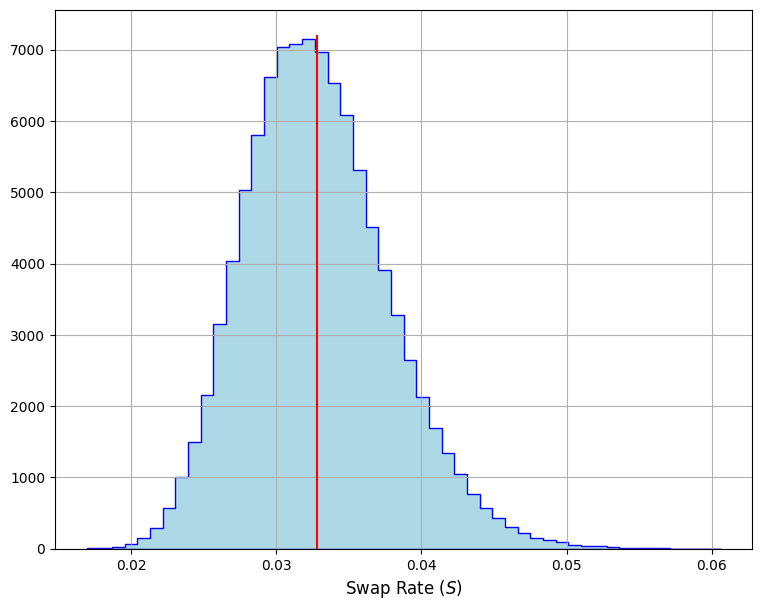
\includegraphics[width=0.55\textwidth]{figures/simulated_swap_rate}
	\caption{Distribution of the simulated swap rate at the exercise date, the spot swap rate is also shown (red line).}
	\label{fig:swap_rate}
\end{figure}

The simulation has been repeated a number of times to check how the swaption NPV changes with the underlying IRS fixed rate $K$. As for plain vanilla European options, when the strike $K$ is much greater then the average simulated swap rate the NPV is almost 0. Conversely when $K$ is much lower the swaption is much valuable. In the intermediate situation where $K$ is close to the average swap rate, the swaption value is influenced by under and over-fluctuation in the simulated swap rate such that there is not a sharp transition between zero and non-zero value.
The results are reported in Fig.~\ref{fig:swaption_npv_vs_K}.

\begin{figure}[htb]
\centering
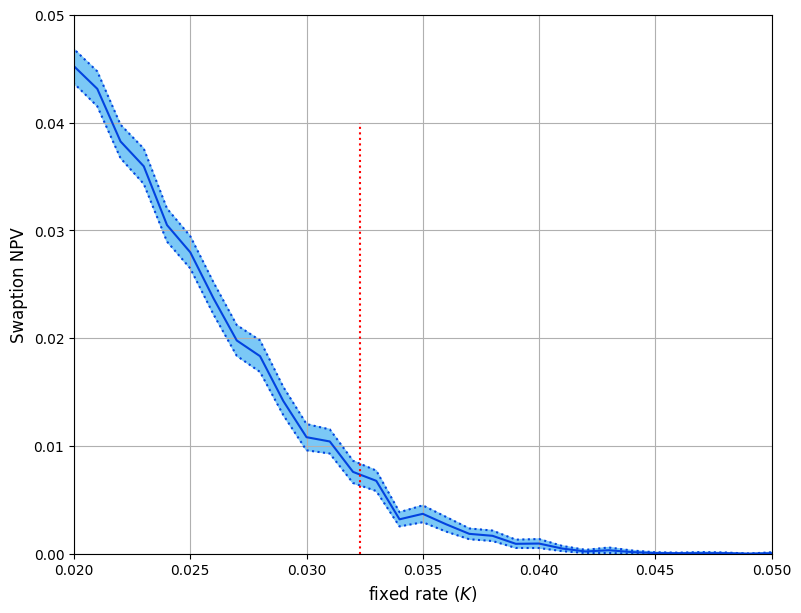
\includegraphics[width=0.6\textwidth]{figures/swaption_npv_vs_K}
\caption{Swaption NPV as a function of the underlying interest rate swap fixed rate $K$.}
\label{fig:swaption_npv_vs_K}
\end{figure}

\section*{Exercises}
\begin{question}
Assume that company A has agreed to pay a 6-month Libor and receive a fixed interest rate of 8\% per year (with interest payable every six months) from the face value of \$100 million. Swap is 1.25 years to expire. The interest rates for 3, 9 and 15 months are: 10\%, 10.5\% and 11\% respectively. Assume that interest rates are continously compounded. The 6-month Libor is currently 10.2\%. 

Calculate the value of this swap for company A.
\end{question}

\cprotEnv\begin{solution}
\begin{ipython}

\end{ipython}
\begin{ioutput}

\end{ioutput}
\end{solution}

\begin{question}
Suppouse that the EURIBOR Forward rates and the discount curve are those defined in
\href{https://github.com/matteosan1/finance_course/blob/develop/libro/input_files/euribor_curve.xlsx}{euribor\_curve.xlsx} and \href{https://github.com/matteosan1/finance_course/raw/develop/libro/input_files/discount_curve.xlsx}{discount\_curve.xlsx} respectively.
Determine the value of an option to pay a fixed rate of 4\% and receives EURIBOR on a 5 year swap starting in 1 year. Assume the notional is 100 EUR, the exercise date is on October, 30th 2020 and the swap rate volatility is 15\%.
\end{question}

\cprotEnv\begin{solution}
\begin{ipython}
import pandas as pd
from finmarkets import InterestRateSwap, ForwardRateCurve
from datetime import date
from dateutil.relativedelta import relativedelta
from scipy.stats import norm
import math

pricing_date = date(2020, 10, 30)
start_date = pricing_date + relativedelta(years=1)
exercise_date = start_date

discount_data = pd.read_excel('discount_curve.xlsx')
euribor_data = pd.read_excel('euribor_curve.xlsx')

dates = [pricing_date + relativedelta(months=i) for i in discount_data['delta']]
dc = DiscountCurve(dates, discount_data.loc[:, 'df'])

dates = [pricing_date + relativedelta(months=i) for i in euribor_data['delta']]
fr = ForwardRateCurve(dates, euribor_data.loc[:, 'rate'])


irs = InterestRateSwap(1e6, start_date, 0.04, 6, 5)
sigma = 0.15
A = irs.annuity(dc)
S = irs.swap_rate(dc, fr)
T = (exercise_date - pricing_date).days / 365
d1 = (math.log(S/irs.fixed_rate) + 0.5 * sigma**2 * T) / (sigma * T**0.5)
d2 = (math.log(S/irs.fixed_rate) - 0.5 * sigma**2 * T) / (sigma * T**0.5)
npv = irs.nominal * A * (S * norm.cdf(d1) - irs.fixed_rate * norm.cdf(d2))

print("Swaption NPV: {:.3f} EUR".format(npv))\end{ipython}
\begin{ioutput}
Swaption NPV: 312218.049 EUR
\end{ioutput}
\end{solution}

%\begin{question}
%A \emph{currency swap}, sometimes referred to as a cross-currency swap, involves the exchange of interest—and sometimes of principal—in one currency for the same in another currency. Interest payments are exchanged at fixed dates through the life of the contract. 
%
%Assume that yield curves in Japan and in the US are flat. The interest rate in Japan is equal to 4\% per annum, and in the US to 9\% per annum (with continuous compounding). A financial institution takes position in a swap contract, under which it receives 5\% on an annual basis of the amount denominated in yen and pays 8\% per annum of the amount denominated in dollars. These amounts are respectively 10 million USD and 1200 million yen. The contract is valid for 3 years and the current exchange rate is 110 USDJPY. What is the value of this currency swap?
%
%\textbf{Hint:} write a \texttt{CurrencySwap} class in order to valuate the swap.
%\end{question}
%
%\cprotEnv\begin{solution}
%\begin{ipython}
%import numpy as np
%
%class CurrencySwap:
%    def __init__(self, amount_for, amount_dom, r_for, r_dom,
%                 fixed_for, fixed_dom, exchg_rate, maturity):
%        self.amount_for = amount_for
%        self.amount_dom = amount_dom
%        self.r_for = r_for
%        self.r_dom = r_dom
%        self.fixed_for = fixed_for
%        self.fixed_dom = fixed_dom
%        self.exchg_rate = exchg_rate # for/dom
%        self.maturity = maturity
%
%    def foreign_npv(self):
%        b_f = 0
%        for t in range(1, maturity+1):
%            b_f += np.exp(-self.r_for*t)*self.fixed_for*self.amount_for
%        b_f += np.exp(-self.r_for*t)*self.amount_for
%        return b_f
%
%    def domestic_npv(self):
%        b_d = 0
%        for t in range(1, maturity+1):
%            b_d += np.exp(-self.r_dom*t)*self.fixed_dom*self.amount_dom
%        b_d += np.exp(-self.r_dom*t)*self.amount_dom
%        return b_d
%
%    def value_dom(self):
%        return self.foreign_npv()/self.exchg_rate - self.domestic_npv()
%
%    def value_for(self):
%        return self.domestic_npv()*self.exchg_rate - self.foreign_npv() 
%\end{ipython}
%\noindent
%\begin{ipython}
%rf = 0.04
%rd = 0.09
%kf = 0.05
%kd = 0.08
%Nf = 1200e6
%Nd = 10e6
%S = 110
%
%cs = CurrencySwap(Nf, Nd, rf, rd, kf, kd, S)
%print ("Domestic Value: {:.0f} USD".format(cs.value_dom()))
%print ("Foreign Value: {:.0f} yen".format(cs.value_for()))
%\end{ipython}
%\begin{ioutput}
%Domestic Value: 1542996 USD
%Foreign Value: -169729535 yen
%\end{ioutput}
%
%The swap value for the financial institution is about 1.54 million USD. If the institution paid in yen and received cash flows in dollars, the swap value would be around -1697 million yen.
%\end{solution}
